\chapter{経路積分から伝播関数と頂点へ}

粒子とその相互作用の目録に移る前に、中心となる構成を明確にしておく価値がある。ラグランジアンは古典場の方程式を符号化するだけにとどまらない。経路積分を通じて、粒子が伝播し、分裂し、結合し、散乱する振幅をも与える。これが量子場の理論からファインマン図への最も直接的な道筋である。

\section{粒子と場の最小作用}

ファインマンの経路積分は最小作用の原理の量子版である。まず、座標と速度に依存するラグランジアンをもつ通常のニュートン粒子から始めよう。
\begin{equation}
\mathcal{L}=\mathcal{L}(x,\dot{x}),
\end{equation}
そして、ある軌道に割り当てられる作用は
\begin{equation}
S[x]=\int \mathcal{L}(x,\dot{x})\,dt.
\end{equation}
である。ある時空点から別の時空点へのあらゆる候補軌道は、ニュートンの方程式を満たすかどうかにかかわらず、作用をもつ。古典軌道は作用が停留的であることによって際立っている。伝統的な``最小作用''の言葉では作用を最小化するが、停留的というのがより一般的な言明である。停留性の条件が古典的な運動方程式を与える。

\begin{figure}[htbp]
\centering
\includegraphics[width=0.72\textwidth]{lecture_10_figure_02.png}
\caption{粒子軌道の作用積分。}
\lectureframe{00:02:14}
\end{figure}

同じ構造が古典場にも当てはまる。すべての場を総称的に\(\phi\)と書く。局所的な場のラグランジアン密度は、場およびその空間微分と時間微分の両方に依存しうる：
\begin{equation}
\mathcal{L}
=\mathcal{L}\!\left(\phi,\frac{\partial\phi}{\partial x^\mu}\right)
=\mathcal{L}(\phi,\partial_\mu\phi).
\end{equation}
相対性理論は\(\mathcal{L}\)がローレンツスカラーとして変換することを要求する。その要件のもとで、場とその微分から作られるスカラー的な組み合わせが、ラグランジアンに可能な項を与える。

\begin{figure}[htbp]
\centering
\includegraphics[width=0.62\textwidth]{lecture_10_figure_03.png}
\caption{場のラグランジアンの場およびその時空微分への依存性。}
\lectureframe{00:04:09}
\end{figure}

場の場合、作用は時空のある領域にわたって積分される：
\begin{equation}
S[\phi]=\int_{\Omega} d^4x\,\mathcal{L}(\phi,\partial_\mu\phi),
\qquad
d^4x=dt\,dx\,dy\,dz.
\end{equation}
粒子の作用は経路に沿った時間についての積分である。場の作用は時空領域全体にわたるラグランジアン密度の積分である。

粒子経路の端点を固定することの類似物は、初期の時間スライスと最終の時間スライス上で完全な場の配置を指定することである。初期の場が\(\phi_{\mathrm{i}}(\mathbf{x})\)で最終の場が\(\phi_{\mathrm{f}}(\mathbf{x})\)ならば、補間する場がその間のスラブ全体を埋める。境界データが古典的な補間解を許すとき、その解は境界配置を固定したもとでの作用の停留点である。
\editorialnote{二つの時間スライス上の任意の完全な場の配置が古典解を許すとは限らない。したがって停留作用の言明は、補間解が存在する境界データに限られる。}

この幾何学は粒子経路の場の理論における対応物である。\footnote{時空スラブはおよそ00：04：29の図から再構成される。}
\begin{figure}[htbp]
\centering
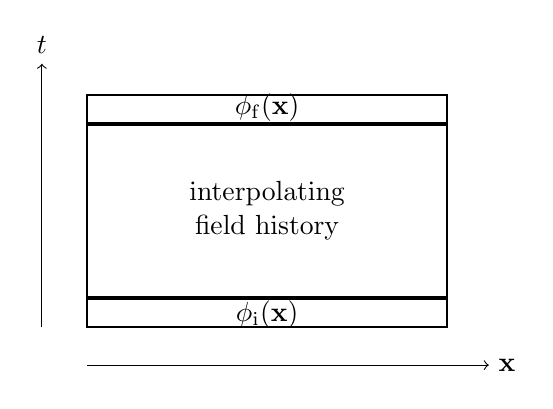
\begin{tikzpicture}[scale=0.88]
\draw[->] (-0.65,0) -- (-0.65,3.8) node[above] {$t$};
\draw[->] (0,-0.55) -- (5.8,-0.55) node[right] {$\mathbf{x}$};
\draw[thick] (0,0) rectangle (5.2,3.35);
\draw[very thick] (0,0.42) -- (5.2,0.42);
\draw[very thick] (0,2.93) -- (5.2,2.93);
\node at (2.6,0.18) {$\phi_{\mathrm{i}}(\mathbf{x})$};
\node at (2.6,3.17) {$\phi_{\mathrm{f}}(\mathbf{x})$};
\node[align=center] at (2.6,1.68) {interpolating\\field history};
\end{tikzpicture}
\caption{時空領域を境界づける初期および最終の場の配置。}
\end{figure}

\begin{classroomqa}
\lecturetimestamp{00:07:34}
\audiencequestion{場は同じ値に戻ることができるか？}
\lecturerresponse{はい。粒子の座標が以前の位置に戻ることに何の障害もないのと同様に、場が以前の値に戻ることに何の障害もない。}
\end{classroomqa}

\begin{classroomqa}
\lecturetimestamp{00:07:46}
\audiencequestion{境界データが場の値であるのに、なぜ時空事象や軌道について語るのか？}
\lecturerresponse{粒子の軌道は場の履歴に置き換えられる。場の空間における各端点は選ばれた時間スライス上の場全体であり、履歴は二つのスライスの間の時空領域の各点における場を指定する。}
\end{classroomqa}

補間する場に停留作用を要求すると偏微分方程式が生じる。場とラグランジアンに応じて、これらにはマクスウェル方程式や、重力作用に対するアインシュタイン方程式のような方程式が含まれる。詳細な変分の導出はここでは不要である；重要な流れは
\begin{equation}
\mathcal{L}
\longrightarrow
S[\phi]
\longrightarrow
\text{classical field equations}.
\end{equation}

\section{ファインマンの粒子経路の和}

量子力学は、どの軌道が起こるかという問いを、振幅についての問いに置き換える。\((x,t)\)に粒子を注入し、しばらく目を閉じ、それから\((x',t')\)で検出器をオンにすることを想像しよう。振幅
\begin{equation}
\mathcal{A}(x,t;x',t')
\end{equation}
は複素数である。その大きさの二乗が確率である：
\begin{equation}
\begin{aligned}
P(x,t;x',t')
&=\left|\mathcal{A}(x,t;x',t')\right|^2\\
&=\mathcal{A}(x,t;x',t')
\mathcal{A}(x,t;x',t')^*.
\end{aligned}
\end{equation}

ファインマンの規則は、あらゆる候補経路に作用を割り当て、それに位相
\begin{equation}
\exp\!\left(-\frac{i}{\hbar}S[x]\right)
=
\exp\!\left[-\frac{i}{\hbar}\int \mathcal{L}(x,\dot{x})\,dt\right].
\end{equation}
を対応させる。

\begin{figure}[htbp]
\centering
\includegraphics[width=0.70\textwidth]{lecture_10_figure_04.png}
\caption{粒子経路に対応する複素位相。}
\lectureframe{00:11:52}
\end{figure}

\(\hbar\) の因子は、指数を無次元にするために必要である。\footnote{00 では、11:52 において、黒板には自然に \(e^{-i\int\mathcal{L}\,dt}\) と書かれており、\(\hbar\) の因子は 00:12:02 での発言で補われる。} 遷移振幅は、端点を結ぶあらゆる可能な経路にわたるこれらの位相の和である：
\begin{equation}
\mathcal{A}(x,t;x',t')
=
\sum_{\substack{\text{paths }x(\tau)\\(x,t)\rightarrow(x',t')}}
\exp\!\left(-\frac{i}{\hbar}S[x]\right).
\end{equation}
ここで ``可能な経路'' とは、ニュートンの方程式の解を意味しない。和に含まれる任意の経路を意味する。非相対論的量子力学では、経路は時間を後ろ向きにループするのではなく前方に進む。プランク定数は作用の次元をもつので、\(S/\hbar\) は無次元である。

指数関数が自然であるのは、連続する小さなステップの振幅が掛け合わされるからである。経路を連続する部分に分割すると、作用は加算され、
\begin{equation}
S=S_1+S_2+\cdots,
\end{equation}
一方、位相は掛け合わされる：
\begin{equation}
e^{-iS/\hbar}
=e^{-iS_1/\hbar}e^{-iS_2/\hbar}\cdots.
\end{equation}
因子 \(i\) は帳簿付けの道具ではなく、量子力学の規則の一部である。

\begin{classroomqa}
\lecturetimestamp{00:13:27}
\audiencequestion{指数関数は、連続する小さなステップの振幅を掛け合わせることと関係しているのか。}
\lecturerresponse{はい。連続するステップの振幅は掛け合わされ、対応する作用の部分は加算される。}
\end{classroomqa}

\begin{classroomqa}
\lecturetimestamp{00:13:49}
\audiencequestion{経路の和そのものが確率なのか。}
\lecturerresponse{いいえ。経路の和は一般に複素数の確率振幅である。それにその複素共役を掛けると確率が得られる。}
\end{classroomqa}

\section{場の履歴にわたる和}

同じ定式化は量子場の理論に拡張されるが、ここでの構成は意図的に非厳密なままにとどめる。初期の場の配位 \(\phi(\mathbf{x})\) と、別に指定された最終の配位 \(\phi'(\mathbf{x})\) から始める。これらは空間の完全な関数であり、二つの孤立した点での値ではない。

すべての空間点で場を準備し、系を発展させ、後ですべての点で場を測定するような理想化された装置を想像してもよい。そのような装置は現実的ではないが、概念的な問いを明確に定義する：初期の完全な場の配位から最終の配位へ移る振幅は何か。

想像しうるあらゆる補間する場の履歴が寄与する。各履歴について、
\begin{equation}
S[\phi]=\int d^4x\,\mathcal{L}(\phi,\partial_\mu\phi)
\end{equation}
を評価し、対応する位相を付ける。概略的には、
\begin{equation}
\mathcal{A}\!\left[\phi(\mathbf{x})\rightarrow\phi'(\mathbf{x})\right]
=
\sum_{\substack{\text{field histories}\\
\phi_{\mathrm{i}}=\phi,\;\phi_{\mathrm{f}}=\phi'}}
\exp\!\left(-\frac{i}{\hbar}S[\phi]\right).
\end{equation}
履歴は古典場の方程式を解く必要はない。それは、介在する時空領域全体にわたる場の値の一つの完全な割り当てにすぎない。

\begin{classroomqa}
\lecturetimestamp{00:17:39}
\audiencequestion{履歴は無限にあり、各々の位相は大きさが1である。それらの和はどのように収束しうるのか。履歴は最小化されているのか。}
\lecturerresponse{履歴は和をとられるのであり、最小化されるのではない。項は単位円の周りに分布する位相であるため、互いに打ち消し合うことができる。これは、ゼロから離れた下限をもつ無限に多くの正の項を加えることとは異なる。振動積分は収束しうる。デルタ関数のフーリエ表示はよく知られた例である。位相が円周上に一様に分布していれば、それらのベクトル和は消える。ほとんどの履歴は強く打ち消し合う。静止作用の軌道の近くの履歴は、そこでは位相の変化が最も遅いため、最も打ち消し合わない。これが古典極限の現れ方である。}
\end{classroomqa}

\editorialnote{実時間の経路積分は通常、収束の処方箋を必要とする。単位円の議論はここで用いられる振動的相殺の議論を与えるものであり、収束の一般的な証明ではない。}

この相殺は複素平面上のベクトル和として描くことができる。\footnote{単位円の作図は00:18:32--00:20:21の板書での議論から再構成した。}
\begin{figure}[htbp]
\centering
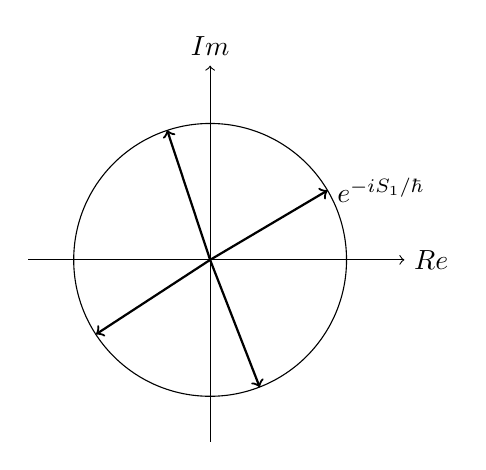
\begin{tikzpicture}[scale=1.05]
\draw[->] (-2.2,0) -- (2.35,0) node[right] {$\operatorname{Re}$};
\draw[->] (0,-2.2) -- (0,2.35) node[above] {$\operatorname{Im}$};
\draw (0,0) circle (1.65);
\draw[thick,->] (0,0) -- (1.42,0.84);
\draw[thick,->] (0,0) -- (-1.38,-0.90);
\draw[thick,->] (0,0) -- (-0.52,1.57);
\draw[thick,->] (0,0) -- (0.60,-1.54);
\node[right] at (1.42,0.84) {$e^{-iS_1/\hbar}$};
\end{tikzpicture}
\caption{単位大きさの位相は、その向きが異なれば相殺しうる。}
\end{figure}

実際、
\begin{equation}
e^{-iS/\hbar}
=
\cos\!\left(\frac{S}{\hbar}\right)
-i\sin\!\left(\frac{S}{\hbar}\right).
\end{equation}
各寄与は単位ベクトルである。異なる向きを指す寄与は、加算すると同時に減算もする。\(S\) の静止点の近くでは、近傍の履歴はほぼ同じ位相をもつため、それらの寄与はより効果的に強め合う。静止作用から離れると、位相は急速に変化し、破壊的干渉が支配する。

この経路積分の構造は、事実上すべての現代の量子場の理論の基礎となっている。次の実践的なステップは、導出するのではなく述べることにする。それは計算への過度に単純化された道筋であるが、同じ対象が二つの言語でどのように用いられうるかを可視化する。

過程を計算するとは、初期状態から最終状態への遷移確率を計算することである。一方の記述は初期の場の配位と最終の場の配位を指定する。もう一方は入射粒子と出射粒子、すなわち1つまたは複数の場の量子を指定する。これらの問いは異なって見えるが、どちらも同じ場の理論の経路積分から計算される。

\section{離散時空形式}

場の履歴の和に具体的な意味を与えるために、時空を小さなセルに分割し、各セルに場の値を割り当てる。連続極限はセルの大きさを縮めることによって近づかれるが、今のところセルは有限のままである。これにより、関数にわたる形式的な和が、格子セルに数値を割り当てることにわたる和へと変換される。

\(1+\mathcal{L}_i\)に似た因子の積を各セルに1つずつ用いる、以前のヒューリスティックな方法があり、次に粒子の伝播と衝突を記述する項を同定する。この構成は繰り返すに値するほど中心的であるが、因子は修正されなければならない。小さな量はラグランジアンそのものではない。それはセルに含まれる作用である。

セルが時空体積
\begin{equation}
a^4=\Delta t\,\Delta x\,\Delta y\,\Delta z,
\end{equation}
を持つなら、その作用は
\begin{equation}
A_i=\mathcal{L}_i a^4.
\end{equation}
である。セルは小さいので、\(A_i\)は小さい。\(\hbar\)を一時的に抑制すると、修正された基本因子は
\begin{equation}
1-iA_i,
\end{equation}
であり、\(1+\mathcal{L}_i\)ではない。

任意の小さな\(\epsilon\)に対して、
\begin{equation}
1+\epsilon\simeq e^\epsilon,
\end{equation}
なぜなら
\begin{equation}
e^\epsilon
=1+\epsilon+\frac{\epsilon^2}{2!}
+\frac{\epsilon^3}{3!}+\cdots.
\end{equation}
であるからだ。したがって、これらの一時的な単位では、十分に小さなセルに対して\(1-iA_i\)は\(e^{-iA_i}\)を近似する。最初から正確な指数因子を用いる方がより簡潔である。

\begin{classroomqa}
\lecturetimestamp{00:27:57}
\audiencequestion{指数関数は\(\hbar\)の因子を必要とするか？}
\lecturerresponse{はい。無次元のセル因子は1次までで\(1-iA_i/\hbar\)であり、正確な指数関数は\(\exp(-iA_i/\hbar)\)である。後で\(\hbar=1\)となる単位を採用してもよい。}
\end{classroomqa}

\(\hbar\)を復元すると、修正された中間因子とその指数関数形は
\begin{equation}
1-\frac{i}{\hbar}A_i
\simeq
\exp\!\left(-\frac{i}{\hbar}A_i\right).
\end{equation}
である。

固定された履歴に対して、時空積分をセル作用の和で置き換える：
\begin{equation}
S[\phi]
=\int d^4x\,\mathcal{L}
\;\longrightarrow\;
\sum_i A_i.
\end{equation}
その履歴の位相は
\begin{equation}
\exp\!\left(-\frac{i}{\hbar}\sum_i A_i\right).
\end{equation}
となる。和の指数関数は指数関数の積である：
\begin{equation}
\exp\!\left(-\frac{i}{\hbar}\sum_i A_i\right)
=
\prod_i\exp\!\left(-\frac{i}{\hbar}A_i\right).
\end{equation}
操作の順序が重要である。まず1つの完全な履歴を選び、そのセル重みを掛け合わせる。その後でのみ、異なる履歴にわたって和を取る。

格子は境界データも明示的にする。\footnote{チェッカーボードとその固定された最初と最後の行は、およそ00：23：54および00：30：49の図から再構成される。}
\begin{figure}[htbp]
\centering
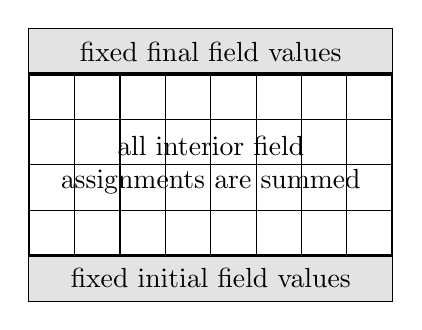
\begin{tikzpicture}[scale=0.72]
\draw[step=0.8,thin] (0,0) grid (6.4,4.8);
\draw[thick] (0,0) rectangle (6.4,4.8);
\fill[gray!22] (0,0) rectangle (6.4,0.8);
\fill[gray!22] (0,4.0) rectangle (6.4,4.8);
\draw[very thick] (0,0.8) -- (6.4,0.8);
\draw[very thick] (0,4.0) -- (6.4,4.0);
\node at (3.2,0.4) {fixed initial field values};
\node at (3.2,4.4) {fixed final field values};
\node[align=center] at (3.2,2.4) {all interior field\\assignments are summed};
\end{tikzpicture}
\caption{初期と最終の格子行が固定された離散場の履歴。}
\end{figure}

最初の行は初期の場の配位を指定し、最後の行は最終の配位を指定する。すべての内部セルには、離散化に含まれるすべての場の値が許される。したがって、遷移振幅は模式的に
\begin{equation}
\mathcal{A}\!\left[\phi_{\mathrm{i}}\rightarrow\phi_{\mathrm{f}}\right]
=
\sum_{\{\phi\}_{\mathrm{interior}}}
\prod_i\exp\!\left(-\frac{i}{\hbar}A_i[\phi]\right),
\end{equation}
の形をとり、最初と最後の行は固定されている。等価的に、各内部配置に対して全作用の指数関数を計算し、その寄与を他のすべての配置からの寄与に加える。

\section{場の配位から粒子の配位へ}

同じ遷移振幅は、場の言葉でも粒子の言葉でも記述できる。最初と最後の時間スライスで場を固定する代わりに、入射する場の量子の集まりと出射する場の量子の集まりを指定し、それらを結ぶ振幅を問うてもよい。評価される対象は同じである。境界の記述だけが変わったのである。

量子場は生成演算子と消滅演算子を含む。したがって場の積は、量子を生成し、消滅させ、または移動させることによって粒子状態に作用する。この演算子としての読み方が、格子経路積分を一連の粒子規則へと変えるのである。

\begin{classroomqa}
\lecturetimestamp{00:34:11}
\audiencequestion{場の量子は必ず粒子として同定できるか？}
\lecturerresponse{別々に観測可能な粒子という従来の意味では、常にそうとは限らない。例えばクォークはクォーク場の量子であるが、閉じ込めのために孤立したクォークが逃げ出して単独で検出されることはない。より一般には、理論で名付けられた場と、従来の観測可能な状態として現れる粒子種との間に一対一の対応がある必要はない。そのような単純な対応を許さない場の理論もある。もし``粒子''が、エネルギーやその他の量子数を運ぶ不可分な量子を広く意味するために用いられるなら、区別は部分的には用語の問題になり得る。}
\end{classroomqa}

\editorialnote{出典の00:35:45--00:36:08における弱結合条件は文法的に曖昧であり、ここでは未解決のままとする。確実に言えるのは、場のラベルと慣習的に観測可能な粒子種が一対一に対応する必要はないということである。}

格子和それ自体は依然として場の値の上を走る。滑らかな古典解に似た配置に制限されるわけではない。

\begin{classroomqa}
\lecturetimestamp{00:36:44}
\audiencequestion{場の履歴は連続でなければならないのか、少なくとも近似的に連続でなければならないのか。}
\lecturerresponse{いいえ。離散格子上では、隣接するセルが単に場の値を持ち、あらゆる割り当てが和に含まれる。近似的に連続な履歴に制限されることはない。量子場は激しく揺らぎ、典型的な履歴は滑らかな古典場ではない。}
\end{classroomqa}

独立に割り当てられる変数は、格子点またはセルにおける場の値である。それらの導関数は隣接する値の差から得られる。

\begin{classroomqa}
\lecturetimestamp{00:37:56}
\audiencequestion{場とその導関数には独立な値が割り当てられるのか。}
\lecturerresponse{いいえ。場の値は格子点に割り当てられる。導関数は隣接する場の値の差から再構成される。異なる有限差分の規約も可能だが、導関数は追加の独立変数ではない。}
\end{classroomqa}

したがって、格子間隔\(a\)に対して、模式的には次のように書ける。
\begin{equation}
\partial_\mu\phi(x)
\longrightarrow
\frac{\phi(x+a\hat\mu)-\phi(x)}{a}.
\end{equation}
場の値の軸自体を小さな区間に分割してもよく、各格子点で可能な値の可算集合が残る。

\begin{classroomqa}
\lecturetimestamp{00:38:53}
\audiencequestion{場が複数あるとき、何が変わるのか。}
\lecturerresponse{各格子点で各場の値が割り当てられ、和はそのようなすべての割り当てにわたって走る。}
\end{classroomqa}

複素数値場を複素変数の解析関数と混同してはならない。解析性は極めて強い滑らかさの条件である。場の経路積分における履歴はそれに従う必要はなく、一般には近似的に滑らかですらない。

\begin{classroomqa}
\lecturetimestamp{00:39:07}
\audiencequestion{場が複素数値であるなら、その値は解析関数が従う滑らかさの条件を満たさなければならないのか。}
\lecturerresponse{いいえ。複素数値であることは解析的であることを意味しない。解析関数の理論は、極めて滑らかで厳しく制約された関数のクラスに関するものである。ここで和をとる場の履歴は位置の解析関数である必要はなく、典型的な履歴は高度に不規則であり、連続極限では高度に不連続とみなしてよい。}
\end{classroomqa}

結果として得られる計算は手に負えないように見える。時空と場の値を離散化した後でも、サンプリングすべき割り当ての数は膨大になりうる。

\begin{classroomqa}
\lecturetimestamp{00:40:04}
\audiencequestion{コンピュータは、どれだけの格子の割り当てをサンプリングすべきか、あるいは計算がいつ収束したかを、どうやって知るのか。}
\lecturerresponse{その問いは格子ゲージ理論、より一般には格子量子場理論に属する。今では効果的な計算分野である。私は格子ゲージ理論の規則を整備する最初の段階に関わったのであって、その後のコンピュータ技術に関わったのではない。規則の整備には約3週間かかったが、こうしたものを計算する技術の開発には30年ほどかかった。実践的な知恵の多くは統計力学から来ており、そこでも分配関数は格子上の配置にわたる和によって得られる---たとえば、結晶中の格子点が占有されているかどうかにわたる和である。十分な配置がサンプリングされたかどうかを判定することは技術的な問題である。専門家は計算が制御下にあるときを知っている---あるいは知っていると思っている---し、得られた計算は実験と一致する。}
\end{classroomqa}

格子ゲージ理論の概念的規則はすぐに得られたが、それらを用いて計算するのに必要な技術にははるかに長い時間がかかった。チェッカーボードは単なる類推ではない。それは実用的な計算手法の出発点でもある。

\section{二次項と粒子の伝播}

ここで場の演算子解釈に戻る。隣接する二つの格子点\(x\)と\(x'\)に対して、積
\begin{equation}
\phi(x)\phi(x')
\end{equation}
は、適切な一粒子行列要素において、一方の格子点での粒子の消滅と他方での生成を与えうる。したがってその粒子セクターでは、1リンクのホップとして描いてよい。これは演算子積の一つの読み方であり、その唯一の意味ではない。

そのような結びつきを担う項は微分項である。厳密に言えば、それらは一つのセルではなく隣接する対に関係づけられる。例えば時間微分は
\begin{equation}
\partial_t\phi(t,\mathbf{x})
\longrightarrow
\frac{\phi(t+a,\mathbf{x})-\phi(t,\mathbf{x})}{a},
\end{equation}
となり、空間微分も空間的リンクに沿って同様に扱われる。

\begin{classroomqa}
\lecturetimestamp{00:44:39}
\audiencequestion{ここで議論しているラグランジアンは二階微分を含むか。}
\lecturerresponse{ここで考察している標準的な理論は一階微分で書かれている。したがってそれらの格子版は隣接サイト間の一階差分を用いる。}
\end{classroomqa}

一階差分を二乗すると、同一サイトの項と隣接クロス項の両方が生じる：
\begin{align}
\frac{1}{2}\bigl[\phi(x)-\phi(x')\bigr]^2
&=
\frac{1}{2}\phi(x)^2
+\frac{1}{2}\phi(x')^2
-\phi(x)\phi(x').
\end{align}
クロス項は一方のサイトから他方への運動を与えることができる。二つの二乗は同一サイトの項である。二次の微分項は運動項であり、伝播を最初に構成するために用いられるのはそれらの隣接クロス項である。

組み合わせ論を分離するために、隣接積を
\begin{equation}
K=\sum_{\langle x,x'\rangle}\phi(x)\phi(x').
\end{equation}
にまとめる。経路積分の重みにおける対応する因子は模式的に
\begin{equation}
e^{-iK}.
\end{equation}
と書かれる。\editorialnote{この模式的な格子因子では、格子間隔の冪\(\hbar\)、計量の符号、規格化定数、およびリンクの係数は省略されている。}
その展開は
\begin{equation}
e^{-iK}
=1-iK-\frac{1}{2!}K^2+\frac{i}{3!}K^3+\cdots,
\end{equation}
であり、あるいは隣接和を露わにすれば
\begin{align}
e^{-iK}
={}&1
-i\sum_{\langle x,x'\rangle}\phi(x)\phi(x')
\nonumber\\
&-\frac{1}{2!}
\sum_{\langle x,x'\rangle}
\sum_{\langle y,y'\rangle}
\phi(x)\phi(x')\phi(y)\phi(y')
+\cdots .
\end{align}
となる。各因子は独立に隣接対を一つ選ぶ。

粒子図はぶら下がり端の規則に従う。露出した端点が許されるのは、境界条件が初期スライスに粒子を明示的に挿入するか、最終スライスから粒子を除去する場合だけである。内部の孤立したリンクは端が不整合であり、指定された遷移への完全な寄与を表さない。内部リンクの端は結合しなければならない。

まず時間層が二つだけの格子を考える。初期状態が\(x\)に粒子を挿入し、最終状態が隣接点\(x'\)でそれを除去するなら、一次の項は二つの境界挿入を結ぶことができる：
\begin{equation}
x\longrightarrow x',
\qquad
\mathcal{A}_{\text{one link}}\sim -i.
\end{equation}
係数\(-i\)はこの模式的展開における係数にすぎず、省略された格子因子と規格化因子は依然として了解されている。

\begin{classroomqa}
\lecturetimestamp{00:52:16}
\audiencequestion{一次の一リンク項は、関係する初期サイトと最終サイトが隣接しているときにのみ寄与するのか。}
\lecturerresponse{はい。その項は隣接対を一つ選ぶので、それらの境界サイトが隣接しているときにのみそれらを結ぶことができる。より遠くへの伝播は高次の積から生じる。}
\end{classroomqa}

二次では、二つの因子が隣接対にわたって独立に和される：
\begin{equation}
K^2
=
\sum_{\langle x,x'\rangle}
\sum_{\langle y,y'\rangle}
\phi(x)\phi(x')\phi(y)\phi(y').
\end{equation}

\begin{classroomqa}
\lecturetimestamp{00:52:40}
\audiencequestion{二番目の隣接対は最初の因子が選んだ対に隣接していなければならないのか。}
\lecturerresponse{いいえ。各因子は独立に隣接対を一つ選ぶ。二つの対はサイトを共有してもよく、完全に別々でもよく、同じ対であってもよい。和はあらゆる可能性を含む。}
\end{classroomqa}

一つの粒子が三つの時間層を伝播する場合、有用な二次の選択は中間サイトを共有する：
\begin{equation}
\bigl[\phi(x_0)\phi(x_1)\bigr]
\bigl[\phi(x_1)\phi(x_2)\bigr],
\qquad
x_0\longrightarrow x_1\longrightarrow x_2.
\end{equation}
最初のリンクの終端は二番目のリンクの始端に結合される。\(x_0\)の初期端点と\(x_2\)の最終端点だけが露出したまま残るので、この項は要求される一粒子遷移に寄与する。模式的な指数関数におけるその係数は
\begin{equation}
-\frac{1}{2!}.
\end{equation}
である。

選択は代わりに別々のホップを形成してもよい。\footnote{リンク図は00:49:18--00:55:12の系列から再構成される。}
\begin{figure}[htbp]
\centering
\resizebox{\linewidth}{!}{%
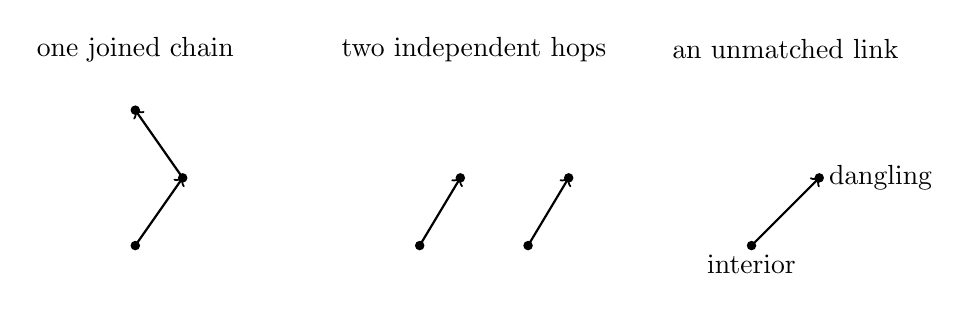
\begin{tikzpicture}[scale=0.86]
\node at (0,2.9) {one joined chain};
\fill (0,0) circle (2pt);
\fill (0.7,1.0) circle (2pt);
\fill (0,2.0) circle (2pt);
\draw[thick,->] (0,0) -- (0.7,1.0);
\draw[thick,->] (0.7,1.0) -- (0,2.0);

\begin{scope}[xshift=4.2cm]
\node at (0.8,2.9) {two independent hops};
\fill (0,0) circle (2pt);
\fill (0.6,1.0) circle (2pt);
\fill (1.6,0) circle (2pt);
\fill (2.2,1.0) circle (2pt);
\draw[thick,->] (0,0) -- (0.6,1.0);
\draw[thick,->] (1.6,0) -- (2.2,1.0);
\end{scope}

\begin{scope}[xshift=9.1cm]
\node at (0.5,2.9) {an unmatched link};
\fill (0,0) circle (2pt);
\fill (1.0,1.0) circle (2pt);
\draw[thick,->] (0,0) -- (1.0,1.0);
\node[below] at (0,0) {interior};
\node[right] at (1.0,1.0) {dangling};
\end{scope}
\end{tikzpicture}%
}
\caption{結合した、独立な、および不整合な隣接リンクの選択。}
\end{figure}

この次数ですでに複数の経路が存在しうる。時間方向と空間方向にそれぞれ一格子ステップだけ変位する場合、二つの順序
\begin{align}
x
&\longrightarrow x+\hat t
\longrightarrow x+\hat t+\hat s,\\
x
&\longrightarrow x+\hat s
\longrightarrow x+\hat s+\hat t
\end{align}
は同じ端点に到達する。

\begin{classroomqa}
\lecturetimestamp{00:55:53}
\audiencequestion{同じ対角端点への別の二ステップ経路はあるか。}
\lecturerresponse{はい。時間ステップを先に取り空間ステップを次に取ることも、逆の順序で取ることもできる。両方の経路が同じ遷移振幅に寄与する。}
\end{classroomqa}

二つのリンクで止める理由はない。三次の項は隣接する三つのリンクの連鎖を与える。経路は直進してもよく、回り道をしてもよく、あるいは遠ざかってから最終点に達する前に戻ってもよい。さらに高次の項には、より長い回り道や繰り返しの後戻りが含まれる。したがって任意の次数まで展開すると、局所的なリンクから組み立てられるあらゆる経路に対する寄与が生じる。点から点への振幅はそれらすべての和であり、その係数には\(i\)の適切な冪と階乗が含まれる：
\begin{equation}
\begin{gathered}
\mathcal{A}(x_{\mathrm{in}}\to x_{\mathrm{out}})
=
\sum_{\text{joined lattice routes }r}c_r,
\\
c_r\ \hbox{read from the exponential expansion}.
\end{gathered}
\end{equation}
係数は一般に複素数であるため、結果として得られる振幅も複素数である。

相対論的な伝播はさらにもう一つの可能性を加える。経路は時間方向に上向きにも下向きにも走ることができ、同じリンクを繰り返し通過することもある。

\begin{classroomqa}
\lecturetimestamp{00:58:47}
\audiencequestion{経路は同じ二つのセルを何度も何度も通過できるのか。}
\lecturerresponse{はい。繰り返しの通過も含まれ、相対論的な展開では経路が時間を遡ることもある。}
\end{classroomqa}

時間を遡る線分は、二つの等価な図形的読み方を許す。時間を遡って走る粒子の線として扱ってもよい。あるいは、時間を前向きにのみ追うならば、粒子--反粒子対が生成され、粒子の側は前進を続け、反粒子は後に元の粒子と出会って消滅する。同じ連結した線が両方の記述を符号化している。\footnote{二つの読み方は00の図と説明に従う：59：00--00：59：51。}

\begin{figure}[htbp]
\centering
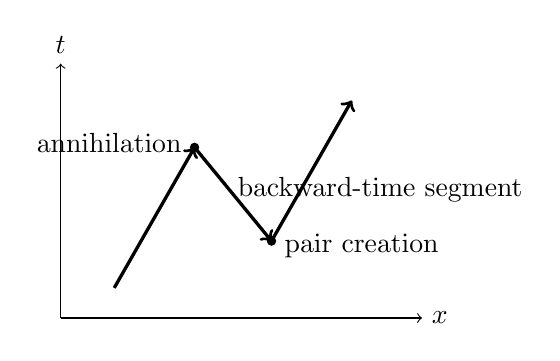
\begin{tikzpicture}[scale=0.85]
\draw[->] (0,0) -- (0,3.8) node[above] {$t$};
\draw[->] (0,0) -- (5.4,0) node[right] {$x$};
\draw[very thick,->] (0.8,0.45) -- (2.0,2.55);
\draw[very thick,->] (2.0,2.55) -- (3.15,1.15);
\draw[very thick,->] (3.15,1.15) -- (4.35,3.25);
\fill (2.0,2.55) circle (2pt);
\fill (3.15,1.15) circle (2pt);
\node[left] at (1.95,2.62) {annihilation};
\node[right] at (3.20,1.08) {pair creation};
\node[right] at (2.50,1.92) {backward-time segment};
\end{tikzpicture}
\caption{時間を遡る線分を前向きに読むと、対生成と対消滅になる。}
\end{figure}

高次に現れる階乗は指数冪級数を制御するが、それは場の配位全体にわたる和を制御することと同じではない。

\begin{classroomqa}
\lecturetimestamp{01:00:00}
\audiencequestion{\(1/n!\)の因子は収束を保証するのか。}
\lecturerresponse{それらは固定された引数に対する指数級数の収束を保証する。それ自体では、すべての場の配位にわたる別個の和の収束を保証しない。これらは別個の問いである。有限格子で場の値が有限個に離散化されている場合、配位の数は有限であるが、連続極限と無限体積極限にはさらなる制御が必要である。}
\end{classroomqa}

\section{一つのリンク積、複数の粒子読み方}

二次の積には一粒子伝播以外のものも含まれる。隣接する二つの対が端点を共有するとき、それは一つの粒子を二リンクの連鎖を通して移動させることができる：
\begin{equation}
\bigl[\phi(x_0)\phi(x_1)\bigr]
\bigl[\phi(x_1)\phi(x_2)\bigr].
\end{equation}
選ばれた対が別々であるとき、同じ二次の項は二つの粒子をそれぞれ一リンクずつ移動させることができる。\footnote{一粒子伝播と二つの独立な一リンクホップの比較は、01での板書の議論から再構成される：00：46--01：02：34。}
\begin{equation}
\bigl[\phi(x_0)\phi(x_1)\bigr]
\bigl[\phi(y_0)\phi(y_1)\bigr],
\qquad x_0\neq y_0.
\end{equation}
第一の因子は一つの粒子を輸送し、第二の因子は別の粒子を輸送する。したがって二次の格子展開には、あらゆる多粒子セクターの伝播振幅が含まれる。同じ代数的次数が、一つのより長い連結経路を記述することも、いくつかのより短い非連結経路を記述することもある。

これは非常に多くの情報であるが、まだ真の相互作用頂点ではない。二次の伝播項だけでは、連結した粒子線が異なる本数の線に分かれることはない。局所的な演算子積がいくつかの生成・消滅の読み方を許すとしても、粒子数を変える過程には追加の相互作用が必要である。

\begin{classroomqa}
\lecturetimestamp{01:03:30}
\audiencequestion{電子と陽電子が消滅して粒子が全く残らないことはあり得るか。}
\lecturerresponse{入射エネルギーが非零で、エネルギーを運ぶ最終状態が存在しない寄与はエネルギー保存則に反する。その可能な時空位置について和をとると、振幅は相殺される。電子--陽電子の消滅は、別の場がエネルギーを運び去るときに起こり得る---例えば電磁量子が生成されるときである。}
\end{classroomqa}

\editorialnote{省略された交換は、二次のホッピングから電子--陽電子消滅へ直接移る。確実な区別は、二次の項は自由伝播を与えるのに対し、物理的な消滅には別の場との相互作用が必要であるということ、そして出力のない振幅はエネルギー保存則によって相殺されるということである。}

したがって微分項は多くのことをなすが、すべてではない。ラグランジアンのさらなる項は、実験的に観測された場の性質と相互作用によって固定される。

\section{質量項}

スカラー場について、ここで議論している微分構造は、模式的に次のローレンツ的符号パターンをもつ。
\begin{equation}
\mathcal{L}_{\mathrm{kin}}
\sim
\frac{1}{2}\left[
(\partial_t\phi)^2
-(\partial_x\phi)^2
-(\partial_y\phi)^2
-(\partial_z\phi)^2
\right].
\end{equation}
この表示は、議論に関係する時間成分マイナス空間成分の構造を定めている。全体の符号と規格化の慣習は暗黙のままにされている。

ラグランジアンは、微分されていない場の冪を含むこともある。二次の例は次の形をとる。
\begin{equation}
\text{mass term}\ \propto\ \frac{1}{2}m^2\phi^2,
\end{equation}
ここで\(m^2\)は質量係数であると同定される。\editorialnote{この箇所では、完全なスカラーラグランジアンの全体の符号の慣習は定められていない。} 模式的な粒子の読みでは、この項は粒子を消滅させ、同じ格子点上で再び生成する。粒子を変位させはしない。経路に同一格子点の因子を挿入する。
\begin{equation}
\text{particle at }x
\longrightarrow
\boxed{m^2\phi(x)^2}
\longrightarrow
\text{particle still at }x.
\end{equation}
そのような挿入が作用するたびに、経路は\(m^2\)に比例する因子をもう一つ獲得する。

微分項のみを残せば、この模式的展開で得られる伝播は質量ゼロの理論である。質量をもつ場では、経路はそのホッピング項の間に任意個の同一格子点の質量挿入を含みうる。質量項は経路の相対的重みを変え、その結果得られる伝播関数が粒子の質量を担うようにする。

\section{三次の項と分裂--履歴の再結合}

質量項は粒子を動かすことなく経路の重みを変える。より興味深い振る舞いは二次より高い次数の項から始まる。三次の相互作用
\begin{equation}
\mathcal{L}_{\mathrm{int}}=g_3\phi^3.
\end{equation}
をとる。一つの格子セルで、三つの場の因子は四つの粒子の読みをもつ。
\begin{equation}
1\longrightarrow 2,
\qquad
2\longrightarrow 1,
\qquad
0\longrightarrow 3,
\qquad
3\longrightarrow 0.
\end{equation}
したがって三次の因子は、一つの粒子を消滅させて二つを生成し、二つを消滅させて一つを生成し、三つを生成し、あるいは三つを消滅させうる。

二次の隣接対の因子は依然として伝播を与える。それらを並べたものは粒子をあるセルまで運び、そのセルでの三次の因子がそれを吸収して二つの粒子を放出し、さらなる二次の因子がそれら二つの粒子を運び去りうる。これは一つの入射粒子と二つの出射粒子をもつ振幅に寄与する。\footnote{格子の幾何は01の図から再構成される。08：48--01：09：42。}

\begin{figure}[htbp]
\centering
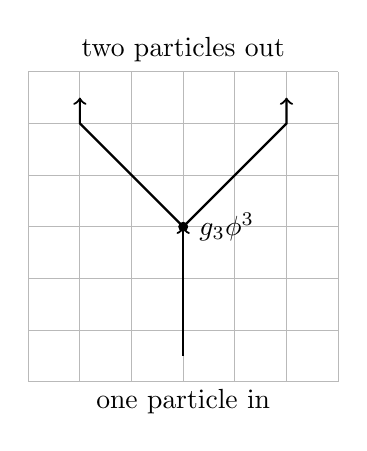
\begin{tikzpicture}[scale=0.82]
\draw[step=0.8,gray!55,thin] (0,0) grid (4.8,4.8);
\draw[thick,->] (2.4,0.4) -- (2.4,1.2) -- (2.4,2.0) -- (2.4,2.4);
\fill (2.4,2.4) circle (2.2pt);
\draw[thick,->] (2.4,2.4) -- (1.6,3.2) -- (0.8,4.0) -- (0.8,4.4);
\draw[thick,->] (2.4,2.4) -- (3.2,3.2) -- (4.0,4.0) -- (4.0,4.4);
\node[right] at (2.5,2.4) {$g_3\phi^3$};
\node at (2.4,-0.3) {one particle in};
\node at (2.4,5.15) {two particles out};
\end{tikzpicture}
\caption{二次の因子は粒子を三次の分裂頂点へと伝播させ、そこから運び去る。}
\end{figure}

最初も最後も一つの粒子である振幅でさえ、もはや単に途切れない単一の経路の和ではない。一つの寄与は二次のホッピングの連鎖による直接的な伝播である。もう一つの寄与は二つの三次の因子を含む。粒子が二つに分裂し、その二つが後に再結合する。したがって中間状態は外部状態よりも多くの粒子を含みうる。\footnote{二つの選択肢は01の図から再構成される。09：44--01：11：36。}

\begin{figure}[htbp]
\centering
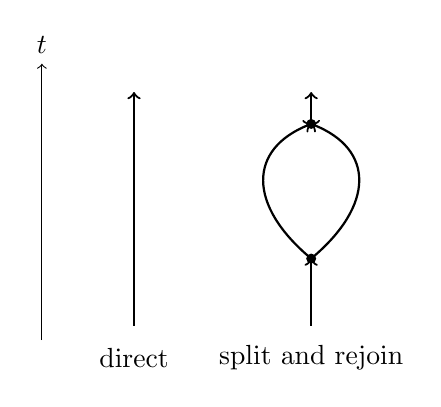
\begin{tikzpicture}[scale=0.9]
\draw[->] (-0.7,0) -- (-0.7,3.9) node[above] {$t$};
\draw[thick,->] (0.6,0.2) -- (0.6,3.5);
\node at (0.6,-0.25) {direct};
\draw[thick,->] (3.1,0.2) -- (3.1,1.15);
\fill (3.1,1.15) circle (2pt);
\draw[thick,->] (3.1,1.15) .. controls (2.2,1.9) and (2.2,2.7) .. (3.1,3.05);
\draw[thick,->] (3.1,1.15) .. controls (4.0,1.9) and (4.0,2.7) .. (3.1,3.05);
\fill (3.1,3.05) circle (2pt);
\draw[thick,->] (3.1,3.05) -- (3.1,3.5);
\node at (3.1,-0.25) {split and rejoin};
\end{tikzpicture}
\caption{同じ一粒子振幅への直接伝播と分裂--再結合の寄与。}
\end{figure}

電気力学における対応する例は、光子を放出し後にそれを再吸収する電子である。その放出と再吸収の履歴は、電子がある点から別の点へ伝播する振幅の一部である。より高次のものは複数の放出と吸収を含む。光子は電子--陽電子対に変換し、その中間対の電子と陽電子がそれ自体光子を交換しうる。初期と最終の粒子内容が単純であるというだけで、中間の粒子内容が単純に見えることを要求するものは何もない。\footnote{以下の再構成における例は01に生じる。11：22--01：12：34。}

\begin{figure}[htbp]
\centering
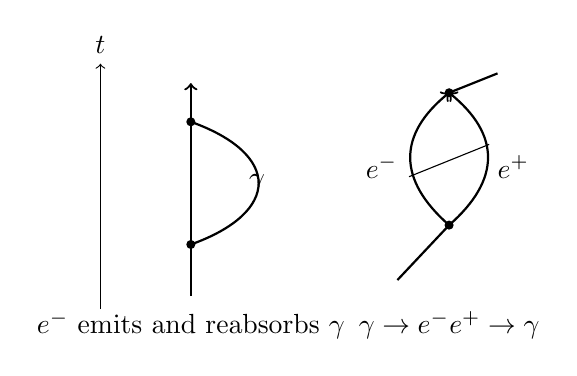
\begin{tikzpicture}[scale=0.82]
\draw[->] (-0.6,0) -- (-0.6,3.8) node[above] {$t$};
\draw[thick,->] (0.8,0.2) -- (0.8,3.5);
\fill (0.8,1.0) circle (2pt);
\fill (0.8,2.9) circle (2pt);
\draw[thick] (0.8,1.0) .. controls (2.2,1.5) and (2.2,2.4) .. (0.8,2.9);
\node[right] at (1.55,1.95) {$\gamma$};
\node at (0.8,-0.25) {$e^-$ emits and reabsorbs $\gamma$};
\draw[thick] (4.0,0.45) -- (4.8,1.3);
\fill (4.8,1.3) circle (2pt);
\draw[thick,->] (4.8,1.3) .. controls (4.0,2.0) and (4.0,2.7) .. (4.8,3.35);
\draw[thick,->] (4.8,1.3) .. controls (5.6,2.0) and (5.6,2.7) .. (4.8,3.35);
\fill (4.8,3.35) circle (2pt);
\draw[thick] (4.8,3.35) -- (5.55,3.65);
\draw[thin] (4.18,2.05) -- (5.42,2.55);
\node[left] at (4.15,2.2) {$e^-$};
\node[right] at (5.4,2.2) {$e^+$};
\node at (4.8,-0.25) {$\gamma\to e^-e^+\to\gamma$};
\end{tikzpicture}
\caption{電子の自己放出の寄与と、電子--陽電子対を含む光子の履歴。}
\end{figure}

そのような履歴のそれぞれは、指数関数の展開における項の確定した積から生じる。その係数は\(i\)の適切な冪、指数級数からの階乗、およびその頂点に付随する結合定数を担う。係数はその履歴の寄与を与えるが、指定された初期状態と最終状態に対する振幅は、それらと同じ外部状態をもつすべての履歴の和である。

\begin{classroomqa}
\lecturetimestamp{01:13:18}
\audiencequestion{同じ全体的な過程がいくつかの異なる履歴で起こり、それらすべてがその振幅に寄与しうるのか。}
\lecturerresponse{はい。その過程の振幅は、同じ初期状態を同じ最終状態に結びつけるすべての異なる履歴から得られる。}
\end{classroomqa}

したがって、量子場の理論を組織する等価な方法が二つある。場の記述では、初期の場の配位と最終の場の配位を指定し、その間のあらゆる場の履歴について和をとる。粒子の記述では、場を量子に分解する。すなわち、入射粒子の内容と出射粒子の内容を指定し、それらをつなぐすべての粒子の履歴を足し合わせる。同じラグランジアンが両方の記述を支配する。

\section{四次項、保存則、結合定数}

四次相互作用
\begin{equation}
\mathcal{L}_{\mathrm{int}}=g_4\phi^4,
\end{equation}
は一点に四つの場の因子をもつ。その局所的な粒子の読みとしては
\begin{equation}
\begin{gathered}
2\longrightarrow2,
\qquad
1\longrightarrow3,
\qquad
3\longrightarrow1,\\
0\longrightarrow4,
\qquad
4\longrightarrow0.
\end{gathered}
\end{equation}
が挙げられる。したがって、単一の四本脚頂点は二粒子散乱、一粒子が三粒子に分裂する過程、三粒子が一粒子に合体する過程、あるいは四本の脚がすべて外向きまたは内向きである過程を記述しうる。\footnote{向きは01:14:28--01:15:18の図から再構成される。}

\begin{figure}[htbp]
\centering
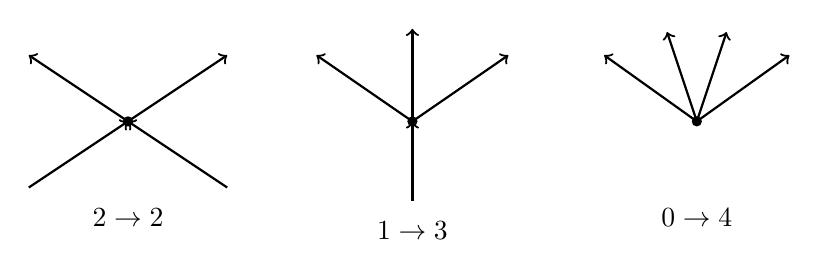
\begin{tikzpicture}[scale=0.84]
\fill (0,0) circle (2.2pt);
\draw[thick,->] (-1.5,-1.0) -- (0,0);
\draw[thick,->] (1.5,-1.0) -- (0,0);
\draw[thick,->] (0,0) -- (-1.5,1.0);
\draw[thick,->] (0,0) -- (1.5,1.0);
\node at (0,-1.45) {$2\to2$};
\begin{scope}[xshift=4.3cm]
\fill (0,0) circle (2.2pt);
\draw[thick,->] (0,-1.2) -- (0,0);
\draw[thick,->] (0,0) -- (-1.45,1.0);
\draw[thick,->] (0,0) -- (0,1.4);
\draw[thick,->] (0,0) -- (1.45,1.0);
\node at (0,-1.65) {$1\to3$};
\end{scope}
\begin{scope}[xshift=8.6cm]
\fill (0,0) circle (2.2pt);
\draw[thick,->] (0,0) -- (-1.4,1.0);
\draw[thick,->] (0,0) -- (-0.45,1.35);
\draw[thick,->] (0,0) -- (0.45,1.35);
\draw[thick,->] (0,0) -- (1.4,1.0);
\node at (0,-1.45) {$0\to4$};
\end{scope}
\end{tikzpicture}
\caption{4本脚の相互作用頂点の3つの局所的向き。}
\end{figure}

局所的な読み\(0\to4\)それ自体は、4つの粒子が物理的過程として真空から現れうるとは述べていない。頂点は依然として、可能なすべての時空位置について和をとらなければならない。提案された外部状態がエネルギーを保存できないとき、それらの位置からの位相は相殺する。

\begin{classroomqa}
\lecturetimestamp{01:15:18}
\audiencequestion{4つが出ていく向きは、最終状態に4つの粒子が自発的に現れることを記述するのか。}
\lecturerresponse{それは4場演算子の一つの局所的な読みであるが、入射エネルギーのない過程はエネルギー保存に反する。頂点の可能なすべての時空位置からの振幅を加えると、それらはゼロに相殺する。}
\end{classroomqa}

\begin{classroomqa}
\lecturetimestamp{01:15:58}
\audiencequestion{エネルギー保存と運動量保存は計算自体から現れるのか。}
\lecturerresponse{はい。頂点をすべての時間について積分するとエネルギー保存が強制され、すべての空間について積分すると運動量保存が強制される。頂点位置についての和は、両方が保存されない限り消える。}
\end{classroomqa}

それらの保存則に従う限り、ラグランジアンによって許されるすべてのグラフがある振幅に寄与する。その寄与の大きさは、各相互作用項の係数に一部依存する。三次と四次の係数を\(G_3\)および\(G_4\)と書く。すべての三本脚頂点は\(G_3\)の因子を一つ寄与し、すべての四本脚頂点は\(G_4\)の因子を一つ寄与する。したがって、\(V_3\)個の三次頂点と\(V_4\)個の四次頂点をもつグラフは、模式的に次の結合定数依存性をもつ
\begin{equation}
\mathcal{A}_{\mathrm{graph}}
\propto G_3^{V_3}G_4^{V_4}.
\end{equation}

これらの結合定数が小さければ、頂点の少ないグラフは一般に頂点の多いグラフより大きく寄与する。頂点が一つ増えるごとに、さらに小さな因子が一つ加わる。これにより摂動和が有用となる可能性が生じる：最も単純なグラフから始め、その後により小さな補正を順次加えていくのである。

完全な級数が実際に収束するかどうかは難しい問題である。結合定数が小さければその順序付けはもっともらしくなるが、それだけですべての収束問題が解決するわけではない。結合定数が大きいと、素朴な級数はまったく破綻するかもしれない。そのような破綻は、基礎となる理論が誤っていることを示すものではない。結合定数の冪での展開がそれを計算するまずい方法であったことを示すだけかもしれない。ここで議論している方法が最も直接的に有用なのは、結合定数が十分小さく、4つの頂点をもつグラフが2つの頂点をもつグラフよりずっと小さい場合である。

\begin{classroomqa}
\lecturetimestamp{01:19:24}
\audiencequestion{カラー理論も同じように扱えるのか。}
\lecturerresponse{はい。カラー理論も同じように定式化でき、後で議論する。}
\end{classroomqa}

\section{伝播関数、頂点、相補的な記述}

次の課題は、粒子を列挙し、その力学をラグランジアンまたはファインマン規則のいずれかで符号化することである。これらは同じ情報の二つの形式である。2次の項は、1点から別の点への伝播を記述する。その伝播を表す線は伝播関数と呼ばれる。3つ以上の場を含む項は、線が出会う場所を記述する。それらの出会い点が頂点である。例えば、
\begin{equation}
\begin{aligned}
\text{quadratic term}
&\longleftrightarrow \text{propagator},\\
G_3\phi^3
&\longleftrightarrow \text{three-leg vertex}.
\end{aligned}
\end{equation}

理論を指定するには、すべての粒子に対して量子場を与え、それらの質量と相互作用をすべて含む1つのラグランジアンを書けばよい。等価に、すべての伝播関数、許されるすべての頂点、および各頂点に付随する係数を列挙してもよい。どちらのリストも、どのような過程が可能であり、それらのグラフに振幅をどのように割り当てるかを教えてくれる。

例えば、2つの電子は光子を交換することで散乱することができる。各電子線は電子--電子--光子頂点を含み、光子伝播関数が2つの頂点を結ぶ。\footnote{この図は01の例から再構成される：21：38。}

\begin{figure}[htbp]
\centering
\begin{tikzpicture}[scale=0.95]
\draw[->] (-0.6,-0.2) -- (0.2,1.4);
\draw[->] (0.2,1.4) -- (-0.7,3.1);
\draw[->] (3.5,-0.2) -- (2.7,1.4);
\draw[->] (2.7,1.4) -- (3.6,3.1);
\fill (0.2,1.4) circle (2pt);
\fill (2.7,1.4) circle (2pt);
\draw[thick] (0.2,1.4) -- (2.7,1.4);
\node[above] at (1.45,1.4) {$\gamma$};
\node[left] at (-0.2,0.5) {$e^-$};
\node[right] at (3.1,0.5) {$e^-$};
\end{tikzpicture}
\caption{光子の交換による2電子散乱。}
\end{figure}

ラグランジアンはこのグラフの振幅を決定し、それを制約する対称性と保存則を含んでいる。時間の向きが定められた図では、下に置かれた粒子が初期配置を形成し、上に置かれた粒子が最終配置を形成する。

\begin{classroomqa}
\lecturetimestamp{01:22:06}
\audiencequestion{ファインマン図において、下にある粒子が初期配置で、上にある粒子が最終配置なのですか。}
\lecturerresponse{はい。下が初期の粒子配置であり、上が最終の粒子配置である。}
\end{classroomqa}

粒子による記述と場による記述は相補的であり、ちょうど通常の量子力学において運動量と位置が相補的な記述であるのと似ている。それらは同じ系を異なる基底で記述している。また、対応する不確定性も存在する。粒子数が精密に指定されれば、場の値は不確定になる。場の値が精密に指定されれば、粒子数は不確定になる。どちらの記述も他方を置き換えるものではなく、ラグランジアンはどちらにおいても有用である。

\begin{classroomqa}
\lecturetimestamp{01:23:26}
\audiencequestion{結合定数は理論によって予言されるのですか、それとも実験によって決定されるのですか。}
\lecturerresponse{対称性は時に一つの結合定数を別の結合定数と関係づけることができるが、その数値は一般に実験から得られる。}
\end{classroomqa}

\section{測定された入力と広範な予言}

量子場の理論それ自体は優雅さと美しさを備えている。しかし、事実を列挙し始めると---どのような粒子が存在するか、その質量はいくらか、その結合定数はいくらか---そのリストは混沌としている。それは非常に醜い混沌であり、対称性によってもたらされる整合性を除けば、ほとんど整合性がない。対称性は異なる種類の粒子とその過程を関係づけるが、限られた範囲においてのみである。その目録の多くは、やや動機づけの乏しい異なる種類の粒子の集合についての、比較的無作為な事実の大きな集まりのままである。

\begin{classroomqa}
\lecturetimestamp{01:24:58}
\audiencequestion{なぜ測定された結合定数はそれほど自信をもって信頼されるべきなのですか。}
\lecturerresponse{いったん結合が測定されれば、それを変えると誤った予言が得られる。その値は、それを用いる多くの計算によって検証される。}
\end{classroomqa}

粒子が多すぎる。つまり場が多すぎる---どんな美的感覚にとっても多すぎる。およそ100個ほどある。結合定数も多く、多かれ少なかれ実験から引き出された数であり、質量も多く、その値はあちこちに広がっている。それらの間にはいくつかの関係があるが、ほんのわずかである。

しかし、いったんそれらを知れば、計算を始めることができる。いったんそれらを知れば、それでおしまいである。それらの粒子についてのどんなことでも、非常に高い精度で計算することができる。クォーク、電子、光子、その他についてのどんなことでも、原子物理学、素粒子物理学、核物理学、化学、そしておそらく生物学にまで及ぶ。入力の量は望ましいよりも多いかもしれないが、出力の量は膨大である。

\section{摂動的な例としての量子電磁力学}

量子電磁力学は結合展開の具体的な例を与える。

\begin{classroomqa}
\lecturetimestamp{01:26:12}
\audiencequestion{電子と光子について、\(G_n\)型の相互作用結合はいくつありますか。}
\lecturerresponse{初等的な相互作用結合は1つある。電荷\(e\)である。それは、電子が入り、電子が出て、光子が放出または吸収される頂点に付随する\(G_3\)型の係数である。}
\end{classroomqa}

スピノル行列と添字を抑制すると、相互作用は模式的な場の内容
\begin{equation}
\mathcal{L}_{\mathrm{QED,int}}
\sim e\,(\text{electron bilinear})\,A,
\end{equation}
を持つ。ここで\(A\)は光子場を表す。詳細なディラック行列の構造は、数え上げの議論には必要ない。QEDの初等的な規則は、電子による光子の放出または吸収である。より複雑なQEDのグラフはすべて、その1つの頂点の繰り返しの使用から組み立てられる。\footnote{模式的な頂点は01から再構成される：26：42。詳細な行列構造は原著では意図的に抑制されている。}

\begin{figure}[htbp]
\centering
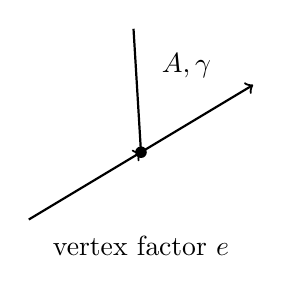
\begin{tikzpicture}[scale=0.95]
\draw[thick,->] (-1.5,-0.9) -- (0,0);
\draw[thick,->] (0,0) -- (1.5,0.9);
\draw[thick] (0,0) -- (-0.1,1.65);
\fill (0,0) circle (2.2pt);
\node[right] at (0.15,1.15) {$A,\gamma$};
\node at (0,-1.25) {vertex factor $e$};
\end{tikzpicture}
\caption{量子電磁力学の初等的な電子--電子--光子頂点。}
\end{figure}

\begin{classroomqa}
\lecturetimestamp{01:27:38}
\audiencequestion{電子--陽子散乱についてはどうか。}
\lecturerresponse{初等的な原子の扱いでは、陽子は固定された無限に重い点源---その場に釘付けにされた重い粒子と理想化できる。陽子自身の量子場のダイナミクスは、陽子と中性子の内部理論を含めるときに初めて入ってくる。}
\end{classroomqa}

\begin{classroomqa}
\lecturetimestamp{01:28:30}
\audiencequestion{電子はその陽子に対して光速に近い速さで運動できるか。}
\lecturerresponse{できる。}
\end{classroomqa}

電子による光子散乱を考える。最低次ではグラフは二つの電子--電子--光子頂点をもつ。したがって振幅は\(e^2\)に比例する：
\begin{equation}
\mathcal{A}_{\mathrm{lowest}}\propto e^2.
\end{equation}
確率、あるいは同等に断面積の結合依存性は、絶対値の二乗から得られ、\(e^4\)に比例する：
\begin{equation}
P_{\mathrm{lowest}}\ \text{or}\ \sigma_{\mathrm{lowest}}
\propto e^4.
\end{equation}
従来の無次元規格化では電気的結合は小さいので、光子が散乱されずにそのまま通過する場合に比べて、真の散乱ははるかに起こりにくい。

この次数ですでに二つのグラフがある。一方の順序では、入射光子が吸収され、出射光子が後で放出される。他方では、出射光子が入射光子の吸収より前に放出される。両方の振幅が寄与する。\footnote{二つの時間順序は01：28：42および01：30：18の図から再構成される。}

\begin{figure}[htbp]
\centering
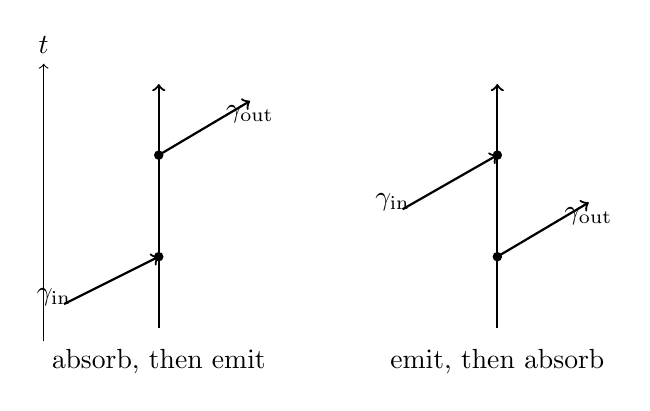
\begin{tikzpicture}[scale=0.86]
\draw[->] (-0.7,0) -- (-0.7,4.1) node[above] {$t$};
\draw[thick,->] (1.0,0.2) -- (1.0,3.8);
\fill (1.0,1.25) circle (2pt);
\fill (1.0,2.75) circle (2pt);
\draw[thick,->] (-0.4,0.55) -- (1.0,1.25);
\draw[thick,->] (1.0,2.75) -- (2.35,3.55);
\node[left] at (-0.15,0.65) {$\gamma_{\mathrm{in}}$};
\node[right] at (1.85,3.35) {$\gamma_{\mathrm{out}}$};
\node at (1.0,-0.3) {absorb, then emit};
\begin{scope}[xshift=5.0cm]
\draw[thick,->] (1.0,0.2) -- (1.0,3.8);
\fill (1.0,1.25) circle (2pt);
\fill (1.0,2.75) circle (2pt);
\draw[thick,->] (1.0,1.25) -- (2.35,2.05);
\draw[thick,->] (-0.4,1.95) -- (1.0,2.75);
\node[right] at (1.85,1.85) {$\gamma_{\mathrm{out}}$};
\node[left] at (-0.15,2.05) {$\gamma_{\mathrm{in}}$};
\node at (1.0,-0.3) {emit, then absorb};
\end{scope}
\end{tikzpicture}
\caption{電子--光子散乱の二つの最低次時間順序。}
\end{figure}

したがって最低次の振幅は一つのグラフではなく、二つの和である：
\begin{equation}
\begin{aligned}
\mathcal{A}^{(2)}
&=
\mathcal{A}_{\mathrm{absorb\ then\ emit}}
+\mathcal{A}_{\mathrm{emit\ then\ absorb}},\\
\mathcal{A}^{(2)}&\propto e^2.
\end{aligned}
\end{equation}

高次補正はさらに多くの素頂点を加える。電子線に二度付く追加の内部光子は\(e\)の因子を二つ加え、振幅では\(e^4\)に比例する寄与を与え、その二乗の大きさでは\(e^8\)を与える。光子線は電子--陽電子挿入を含むこともでき、これもまた素頂点と\(e\)の追加の冪を加える。これらは例であり、網羅的なリストではない。余分な光子は多くの位置に付きうる。\footnote{高次構造は01：30：38--01：31：16から再構成される。}

\begin{figure}[htbp]
\centering
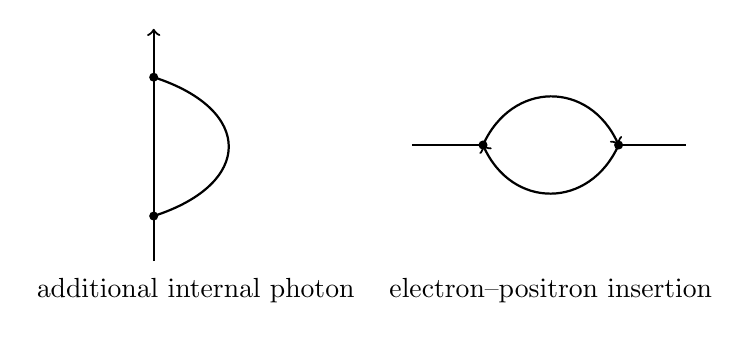
\begin{tikzpicture}[scale=0.82]
\draw[thick,->] (0.9,0.2) -- (0.9,3.8);
\fill (0.9,0.9) circle (2pt);
\fill (0.9,3.05) circle (2pt);
\draw[thick] (0.9,0.9) .. controls (2.45,1.4) and (2.45,2.55) .. (0.9,3.05);
\node at (1.55,-0.25) {additional internal photon};
\begin{scope}[xshift=5.1cm]
\draw[thick] (-0.2,2.0) -- (0.9,2.0);
\fill (0.9,2.0) circle (2pt);
\fill (3.0,2.0) circle (2pt);
\draw[thick,->] (0.9,2.0) .. controls (1.35,3.0) and (2.55,3.0) .. (3.0,2.0);
\draw[thick,->] (3.0,2.0) .. controls (2.55,1.0) and (1.35,1.0) .. (0.9,2.0);
\draw[thick] (3.0,2.0) -- (4.05,2.0);
\node at (1.95,-0.25) {electron--positron insertion};
\end{scope}
\end{tikzpicture}
\caption{素頂点と\(e\)のさらなる冪を加える二つの高次QED構造。}
\end{figure}

したがってQEDの展開は\(e^2\)の逐次の冪で進む。同程度の新たな複雑化はそれぞれ、振幅に電気電荷の二つの冪を加える。用いている規格化では、それによりそのような補正は振幅において前の次数よりおよそ百倍あるいは二百倍小さくなる。より複雑なグラフは次第に弱くなるので、摂動的な和は有用である見込みをもつ。

確率は各グラフを別々に二乗してからそれらの二乗を足すことでは得られない。まず同じ外部過程に寄与するすべての振幅を足す：
\begin{equation}
\mathcal{A}_{\mathrm{total}}=\sum_r\mathcal{A}_r.
\end{equation}
その後に初めて
\begin{equation}
P=\left|\mathcal{A}_{\mathrm{total}}\right|^2
=\left|\sum_r\mathcal{A}_r\right|^2.
\end{equation}
を作る。異なるグラフ間の交差項は干渉項である。規則は単純かつ本質的である：まず足し、次に二乗する。

\section{粒子の目録と標準模型に向けて}

伝播関数、頂点、結合の数え上げ、干渉が揃ったので、素粒子物理学の記述を本格的に始められる。粒子に名前を付け、その質量を指定し、それらを支配するラグランジアンを一部は理論から一部は実験から書き、それらの対称性をそのラグランジアンにおいて直接調べることができる。同じ枠組みが次に標準模型とその性質へと導く。

\begin{classroomqa}
\lecturetimestamp{01:33:22}
\audiencequestion{定数の質量係数\(m^2\)をヒッグス場で置き換えられるか。}
\lecturerresponse{できる。それが正しい考えであり、その機構は後で議論する。}
\end{classroomqa}

\begin{classroomqa}
\lecturetimestamp{01:33:42}
\audiencequestion{隣接する格子点\(x\)と\(x'\)は二つの異なる時刻に位置できるか。}
\lecturerresponse{できる。それらは時間方向の隣接点でありうる。格子における縦方向の伝播はそのように表される。}
\end{classroomqa}

隣接点に対して、有限差分の二乗は同一サイト項と交差リンク項の両方を含む：
\begin{equation}
\bigl[\phi(x)-\phi(x')\bigr]^2
=
\phi(x)^2+\phi(x')^2-2\phi(x)\phi(x').
\end{equation}

\begin{classroomqa}
\lecturetimestamp{01:33:56}
\audiencequestion{どの項が単に静止している粒子を表すか。}
\lecturerresponse{有限差分の二乗における同一サイト項\(\phi(x)^2\)と\(\phi(x')^2\)は静止を表し、交差項\(\phi(x)\phi(x')\)が運動の解釈を与える。明示的な質量項も同一サイトの静止因子に寄与する。}
\end{classroomqa}
